\documentclass[12pt]{article}

\usepackage{amsmath}
\usepackage{amsthm}
\usepackage{amssymb}
\usepackage{fancyhdr}
\usepackage{tikz}
\usepackage{float}
\pagestyle{plain}

\tikzset{node distance=3cm, auto}

\author{Evgeny Kotelnikov}
\title{Exercises for Chapter 2}
\date{}

\begin{document}
\maketitle

\begin{enumerate}

  \item[4.]
    \begin{enumerate}
      \item[a.]
        Basically, we are asked to prove, that monomorphisms, epimorphisms and isomorphisms are closed under composition.

        \begin{center}
          \vspace{-1.75em}\line(1,0){335}
        \end{center}

        Let $f : A \rightarrowtail B$ and $g : B \rightarrowtail C$. Suppose $h$ is not \emph{monic}, that is, there are $p, q : D \to A$, such that $h \circ p = h \circ q$ and $p \neq q$. Since $h = g \circ f$,
        \begin{equation}
          \label{eq:pfg=qfg}
          g \circ f \circ p = g \circ f \circ q.
        \end{equation}
        Since $g$ is \emph{monic} and \ref{eq:pfg=qfg},
        \begin{equation}
          \label{eq:pf=qf}
          f \circ p = f \circ q.
        \end{equation}
        Since $f$ is \emph{monic} and \ref{eq:pf=qf},
        \begin{equation*}
          p = q.
        \end{equation*}
        Contradiction, therefore $h$ is \emph{monic}.

        \begin{center}
          \vspace{-1.75em}\line(1,0){335}
        \end{center}

        Let $f : A \twoheadrightarrow B$ and $g : B \twoheadrightarrow C$. Suppose $h$ is not \emph{epic}, that is, there are $i, j : C \to D$, such that $i \circ h = j \circ h$ and $i \neq j$. Since $h = g \circ f$,
        \begin{equation}
          \label{eq:fgi=fgj}
          i \circ g \circ f = j \circ g \circ f.
        \end{equation}
        Since $f$ is \emph{epic} and \ref{eq:fgi=fgj},
        \begin{equation}
          \label{eq:gi=gj}
          i \circ g = j \circ g.
        \end{equation}
        Since $g$ is \emph{epic} and \ref{eq:gi=gj},
        \begin{equation*}
          i = j.
        \end{equation*}
        Contradiction, therefore $h$ is \emph{epic}.

        %\begin{center}
        %  \line(1,0){250}
        %\end{center}

        Let $f : A \to B$ and $g : B \to C$ be \emph{iso}. Therefore, there are arrows $f^{-1} : B \to A$ and $g^{-1} : C \to B$ such that
        \begin{align}
          \label{eq:f-1f=1A} f^{-1} \circ f &= 1_A, \\
          \label{eq:ff-1=1C} f \circ f^{-1} &= 1_B, \\
          \label{eq:g-1g=1B} g^{-1} \circ g &= 1_B, \\
          \label{eq:gg-1=1C} g \circ g^{-1} &= 1_C. 
        \end{align}
        Let $h' = f^{-1} \circ g^{-1}$. From \ref{eq:f-1f=1A} it follows that $f^{-1} \circ 1_B \circ f = 1_A$. From \ref{eq:g-1g=1B} it follows that $f^{-1} \circ g^{-1} \circ g \circ f = 1_A$, therefore $h' \circ h = 1_A$.
        
        Similarly, from \ref{eq:gg-1=1C} it follows that $g \circ 1_B \circ g^{-1} = 1_C$. From \ref{eq:ff-1=1B} it follows that $g \circ f \circ f^{-1} \circ g^{-1} = 1_C$, therefore $h \circ h' = 1_C$.

        $h \circ h' = 1_C$ and $h' \circ h = 1_A$, therefore $h' = h^{-1}$ and $h$ is \emph{iso}.
      \item[b.]
        Let $h : A \rightarrowtail C$. Suppose $f : A \to B$ is not \emph{monic}, that is, there are $p, q : D \to A$, such that
        \begin{equation}
          \label{eq:fp=fq}
          f \circ p = f \circ q
        \end{equation}
        and $p \neq q$. From \ref{eq:fp=fq} it follows that $g \circ f \circ p = g \circ f \circ q$. Since $h = g \circ f$, $h \circ p = h \circ q$. At the same time $h$ is \emph{monic}, therefore $p = q$. Contradiction, therefore $f$ is \emph{monic}.
      \item[c.]  
        Let $h : A \twoheadrightarrow C$. Suppose $g : B \to C$ is not \emph{epic}, that is, there are $i, j : C \to D$, such that
        \begin{equation}
          \label{eq:ig=jg}
          i \circ g = j \circ g
        \end{equation}
        and $i \neq j$. From \ref{eq:ig=jg} it follows that $i \circ g \circ f = j \circ g \circ f$. Since $h = g \circ f$, $i \circ h = j \circ h$. At the same time $h$ is \emph{epic}, therefore $i = j$. Contradiction, therefore $g$ is \emph{epic}.
      \item[d.]
        In the category of sets let $A = C = \{0\}$, $B = \{0, 1\}$ and all arrows constantly $0$. $h : A \to C$ is \emph{monic}, whereas $g : B \to C$ is not.
    \end{enumerate}

  \item[7.]
    Let $A$ be a retract of $P$, that is, there exists $r : P \to A$ and $s : A \to P$ such that \begin{equation}\label{eq:7rs=1} r \circ s = 1_A.\end{equation} To prove that it's projective we need to show that for every $e : X \twoheadrightarrow Y$ and $f : A \to Y$ there exists $\bar{f} : A \to X$ such that $e \circ \bar{f} = f$.

    Let $g = f \circ r$. By projectivity of $P$ there exists $\bar{g} : P \to X$ such that $$e \circ \bar{g} = g = f \circ r.$$

    Composing both sides with $s$ we get $$e \circ \bar{g} \circ s = f \circ r \circ s.$$

    From 11 it follows that $$e \circ \bar{g} \circ s = f \circ 1_A = f.$$

    Asserting $\bar{f} = \bar{q} \circ s$ we get $e \circ \bar{f} = f$, effectively proving desired property.

    \begin{figure}
      \centering
      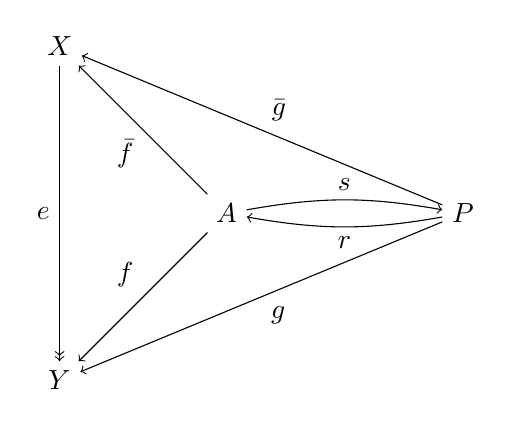
\begin{tikzpicture}
        \node (P)              {$P$};
        \node (A) [left of=P] {$A$};
        \node (X) [above left of=A] {$X$};
        \node (Y) [below left of=A] {$Y$};

        \draw[->] (P) to[bend left=10] node {$r$} (A);
        \draw[->] (A) to[bend left=10] node {$s$} (P);

        \draw[<-] (Y) to node {$f$} (A);
        \draw[->] (A) to node {$\bar{f}$} (X);

        \draw[<-] (X) to node {$\bar{g}$} (P);
        \draw[->] (P) to node {$g$} (Y);

        \draw[<<-] (Y) to node {$e$} (X);
      \end{tikzpicture}
    \end{figure}

    %Let $P$ be a projective object, that is, for any $e : E \twoheadrightarrow X$ and $f : P \to X$ there is some $\overline{g} : P \to E$ such that $e \circ \overline{g} = g$. To show that its retract $Q$ is projective, we have to prove, that for any $h : Q \to X$ there is some $\overline{h} : P \to E$ such that $e \circ \overline{h} = h$. Let $f : Q \to P$ be \emph{iso}. There holds that $g \circ f = h$ and, considering projectivity of $P$, $e \circ \overline{g} \circ f = h$. Asserting $h' = \overline{g} \circ f$ yields desired property.

  \item[13.]
    We will prove that products are associative up to isomorphism.
    \begin{figure}[H]
      \centering
      \begin{tikzpicture}
        \node (A)                      {$A$};
        \node (A*B)   [right of=A]     {$A \times B$};
        \node (B)     [right of=A*B]   {$B$};
        \node (A*B*C) [below of=A*B]   {$(A \times B) \times C$};
        \node (C)     [below of=A*B*C] {$C$};
        
        \draw[<-] (A) to node {$p_1$} (A*B);
        \draw[->] (A*B) to node {$p_2$} (B);
        \draw[->] (A*B*C) to node {$p_3$}           (A*B);
        \draw[->] (A*B*C) to node {$p_1 \circ p_3$} (A);
        \draw[<-] (B) to node {$p_2 \circ p_3$} (A*B*C);
        \draw[<-] (C) to node {$p_4$}           (A*B*C);

        \node (A2)     [right of=B]      {$A$};
        \node (A*B*C2) [below of=A2]     {$A \times (B \times C)$};
        \node (B*C)    [below of=A*B*C2] {$B \times C$};
        \node (B2)     [left  of=B*C]    {$B$};
        \node (C2)     [right of=B*C]    {$C$};

        \draw[<-] (A2) to node {$q_4$} (A*B*C2);
        \draw[<-] (B2) to node {$q_1 \circ q_3$} (A*B*C2);
        \draw[->] (A*B*C2) to node {$q_2 \circ q_3$} (C2);
        \draw[->] (A*B*C2) to node {$q_3$} (B*C);
        \draw[->] (B*C) to node {$q_1$} (B2);
        \draw[<-] (C2) to node {$q_2$} (B*C);

        \draw[dashed,->] (A*B*C2) to[bend right=10] node[above] {$i$} (A*B*C);
        \draw[dashed,->] (A*B*C) to[bend right=10] node[below] {$j$} (A*B*C2);
      \end{tikzpicture}
    \end{figure}

    Since $(A \times B) \times C$ is a product, there exists a unique arrow $$i : A \times (B \times C) \to (A \times B) \times C$$ such that
    \begin{align*}
                q_4 &= p_1 \circ p_3 \circ i, \\
      q_1 \circ q_3 &= p_2 \circ p_3 \circ i, \\
      q_2 \circ q_3 &= p_4 \circ i.
    \end{align*}

    Similarly, since $A \times (B \times C)$ is a product, there exists a unique arrow $$j : (A \times B) \times C \to A \times (B \times C)$$ such that
    \begin{align*}
      p_1 \circ p_3 &= q_4 \circ j,\\
      p_2 \circ p_3 &= q_1 \circ q_3 \circ j,\\
                p_4 &= q_2 \circ q_3 \circ j.
    \end{align*}

    Composing, $q_4 = q_4 \circ j \circ i$ and $p_4 = p_4 \circ i \circ j$. Since also $q_4 \circ 1_{A \times (B \times C)} = q_4$, it follows from the uniqueness condition that $j \circ i = 1_{A \times (B \times C)}$. It can similarly be proved that $i \circ j = 1_{(A \times B) \times C}$. Therefore, both $i$ and $j$ are isomorphisms and $A \times (B \times C) \cong (A \times B) \times C$.

\end{enumerate}

\end{document}
